% $Id: gui_bmodel.tex 395 2011-11-17 22:34:59Z cphillip $

\chapter{Computing Feature and Region Contributions}
\label{chap:ComputeWeights}

\minitoc

\section{Introduction}

The previous modules allow the user to specify one or more models. These include the machine to be used, the cross-validation scheme and the classification/regression problem. The estimation of those models led to predictions on unseen/test data (in each fold), from which measures of performance of the model can be derived and displayed.
\\

In addition, as PRoNTo uses linear models it provides the option of recovering the model weights in the original feature space, and transforming the weights vector into an image, or map. These maps contain at each feature the corresponding weight of the linear model (that together define the predictive function), and which related to how much this particular feature contributed to the classification/regression task in question. The weights can later be displayed using the `Display weights' modules (described below).
\\

Furthermore, the MKL machine estimates contribution of each kernel to the predictive function. This means that there will be one value per region of interest as defined by an atlas and/or per modality (depending on how multiple kernels were built). Therefore, it is possible to build maps at the kernel level, in addition to the maps at the feature level. Kernels (which can correspond to different regions, different channels or different modalities) can then be ranked according to their contribution to the model. Since L1-MKL is a sparse algorithm, only a subset of the kernels will have a non-null contribution to the model, this can facilitate model interpretation.
\\

If the user wants to create images of the weights, using the GUI, the user first needs to click the `Compute weights' button on the main PRoNTo window. This will launch the window shown in Fig \ref{CompWeights}. To estimate the weights and create the weight maps the user needs to select a {\tt PRT.mat} file. The window is then divided in two panels: a `Feature weights' panel and a `Atlas-based weights' panel which are further explained in the sections below.
\\[1cm]

\begin{figure}[h!]
\begin{center}
	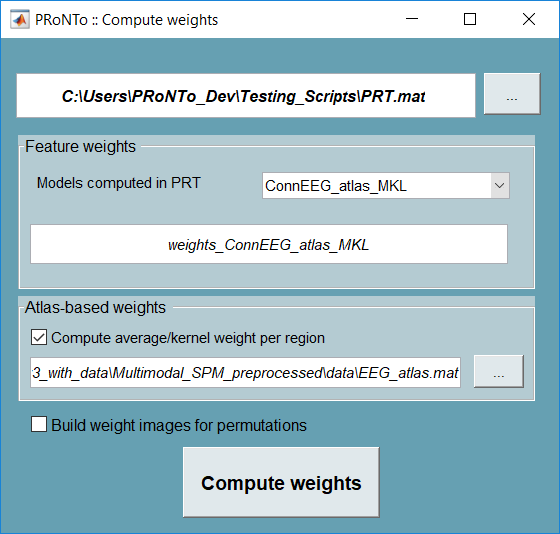
\includegraphics[height=9cm]{images/Tutorial/v3/multimodal_face_gui_compute_weights_ConnEEG_atlas_MKL.png}
	\caption{Weights computation in GUI.}
	\label{CompWeights}
\end{center}
\end{figure}


\section{Feature weights}

For kernel methods the weights can be estimated as a linear combination of the training examples. For non-kernel algorithms the weights are directly computed and saved in the PRT structure. For the kernel algorithms PRoNTo saves the coefficients of the training examples. These coefficients are then multiplied by the training examples to obtain the model weights. The vector of model weights has the same dimensions of the original feature space. In case of NIfTI and MEEG data the model weights can be converted to an image with the same dimensions of the input images. This computation is done for each fold. If for example we have standard MRI data which have 3 dimensions, then the weights can be converted to a 3D image. The resulting 3D images for all folds are then assembled into a single 4D NIfTI file with dimensions [3D x (number of folds + 1)], where $1$ corresponds to an extra 3D image with the averaged weights over all folds. The NIfTI file is saved in the same directory as PRT.mat. In the case of multi-class classification, one image will be built for each class, the index of the class being saved in the image name (e.g. \textit{image\_ name\_ c1.img}). In the case of multiple modalities being considered as multiple kernels (i.e. not concatenated in samples), one image will be built for each modality, the modality name being appended to the image name. In case of data of lower dimensions, for example MEEG data in sensor space (2D), as well as data in a .mat file format, the procedure remains the same.
\\

In the `Feature weights' panel, PRoNTo will show the list of available models, and the user can choose one model for which to estimate the weights. If the selected model is the MKL modelling of ROI-based kernels, the `Atlas-based weights' panel will be automatically updated, and the name of the selected atlas at the feature set step will appear. Otherwise, those fields will stay blank.
\\

In this panel, it is also possible to define the name of the created image file, which is saved in the same directory as PRT.mat. Alternatively, if left empty, PRoNTo will name the file according to the model name, class (if multi-class machine) and/or modality (if MKL on modalities).
\\[1.5cm]

\section{Atlas-based weights}

The `Atlas-based weights' panel allows the user to estimate the contribution to the model, of each anatomically defined region of interest (ROI), as defined by an atlas (same dimensions as for the feature weight images). If the model refers to an MKL machine estimated on kernels per region, the `Atlas name' field will be filled automatically and the contribution of each region is derived from the contribution of each kernel (i.e. they correspond to the kernel weights). If this is not the case (single kernel machine or feature set), an atlas should be loaded (using the browse option). The weights will then be summarized for each region a posteriori. 

Two options are available when estimating such contributions:

\begin{itemize}
\item Contributions of kernels estimated through MKL: In this case, the contributions of each region to the model are derived from the contributions of each kernel. This option is available for MKL modelling of feature sets containing multiple kernels based on ROIs defined by an atlas.

\item Summarizing the weights according to ROIs: If, for example we have MRI data and a whole brain feature set was used, or if the kernels were added to perform single kernel modelling (e.g. SVM, GP, KRR, RVR), it is possible to select an atlas and summarize a posteriori the weights in each anatomically defined ROI. The contribution of each region is then simply the sum of the absolute values of the weights within that region, divided by the number of voxels (or features in general) in that region (see \cite{Schrouff2013a} for details). If summarizing weights by using an atlas is desired, this atlas should be used as a second level mask in the `feature set' step to ensure a perfect overlap between the atlas and the model features. Otherwise, any voxels used as features (or features used in general) in the model but not present in the atlas will be summarized in one extra region referred to as `other' that will not correspond to any anatomical region.
\end{itemize}

In both cases, the contribution of each region is divided by the total contribution of all regions. The derived values can then be seen as percentages of contribution of each region to the decision function. The contributions can be ranked, leading to a list of regions sorted by descending contribution to the model. This list can also be computed if multiple modalities were built and used in an MKL model. In this case, each modality has a contribution to the model, that can be normalized and a sorted list can be derived.
\\

Furthermore, for MKL models - which are sparse in the number of kernels contributing to the model - a bar graph can be built, representing the number of kernels with a non-null contribution to the model. The same graph bar will depict the contribution of each region to the decision function in the case of summarized weights. In this case, the bar graph will not be sparse.
\\

Finally, from PRoNTo v3.0, there is also a new button below the `Atlas-based weights' panel, named `Build weight images for permutations' which when checked, enables to build weight images for each permutation independently. % This allows for statistical tests to be performed on weights and/or on the derived ranking of the regions (for MKL modelling of anatomically defined ROIs).








\section{Batch interface}

The {\tt matlabbatch} module to compute the weights has the same options as the GUI. One main difference being that instead of listing the available models in a given PRT, it will ask for the name (string) of the model to be used. As for estimating models, the name of the model should be exactly the name given in `Model: Specify new/from'. % Another difference is that the batch allows to compute weight images for each permutation. In this case, only the average across folds will be saved in a NIfTI. This potentially allows for statistical tests to be performed on weights and/or on the derived ranking of the regions (for MKL modelling of anatomically defined ROIs).

\begin{figure}[h!]
\begin{center}
	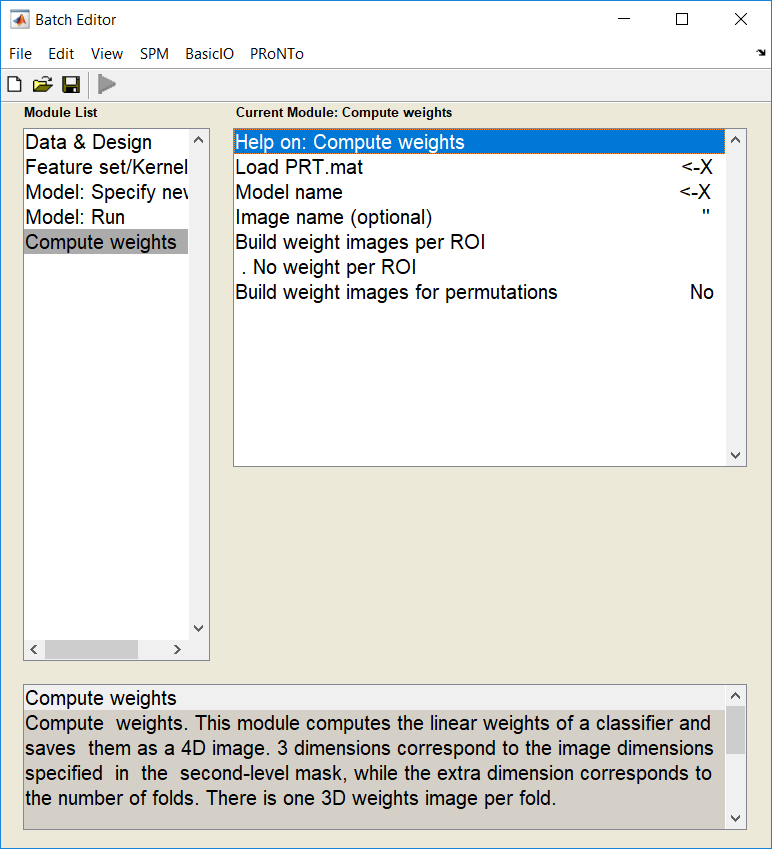
\includegraphics[height=10cm]{images/Tutorial/v3/batch_compute_weights.png}
	\caption{Weights computation in {\tt matlabbatch}.}
	\label{batch_CompWeights}
\end{center}
\end{figure}
